% Other chapters:
%
% PKE and Security Notions			Nuttapong Attrapadung & Takahiro Matsuda
% Advanced Encryption (IBE, ABE, FE, etc)	Romain Gay
% Broadcast Encryption & Traitor Tracing	Duong Hieu Phan
% Signatures and Security Notions		Marc Fischlin
% Advanced Signatures				Olivier Sanders
% E-cash					Georg Fuchsbauer
% ZK Proofs					Ivan Visconti
% SNARGs & Verifiable Computations		Dario Fiore
% Key Exchange					Colin Boyd
% Password-Authenticated Key Exchange		Stas Jarecki
% MPC & Distributed Cryptography		Yehuda Lindell
% Cryptanalysis					Phong Nguyen
% Pairing-based Crypto				Olivier Blazy
% Isogeny-based Crypto				Luca De Feo

\def\Z{\mathbb{Z}}
\def\Q{\mathbb{Q}}
\def\F{\mathbb{F}}
\def\Gal{\mathrm{Gal}}
\def\End{\mathrm{End}}
\def\Ell{\mathrm{Ell}}
\def\Cl{\mathrm{Cl}}
\def\O{\mathcal{O}}
\def\abs#1{|#1|}
\def\polylog{\mathrm{polylog}}
%\def\exp{\mathrm{exp}}
%\def\com{\mathcal{C}}

\chapter{Isogeny Based Cryptography}
\authorname{Luca De Feo}{IBM Research Z�rich}

Isogenies are morphisms of elliptic curves, it thus shouldn't be
surprising that they have played an important role since the early
days of Elliptic (and Hyperelliptic) Curve Cryptography. %
In the 90's, already, they were used to speed up elliptic curve point
counting algorithms~\cite{schoof85,atkin91,atkin92,elkies92,schoof95},
a fundamental tool to set up parameters for elliptic curve
cryptosystems. %
In the last century, \emph{isogeny graphs} were used to show the
random reducibility of discrete logarithm problems within an
\emph{isogeny class}~\cite{AC:JaoMilVen05,jao+miller+venkatesan09},
and related
applications~\cite{Gal,EC:GalHesSma02,teske06,galbraith+stolbunov11}.

Isogeny Based Cryptography is the subbranch of Elliptic Curve
Cryptography researching \emph{constructive} applications of
isogenies.  %
Its distinguishing feature is that the security of its cryptosystems
does not rely on the discrete logarithm problem. %
Its roots go back to Couveignes' seminal ``Hard Homogeneous Spaces''
unpublished work~\cite{EPRINT:Couveignes06}, which sought to establish
a generalization of the discrete logarithm problem. %
Early isogeny based systems include Charles, Goren and Lauter's
collision-resistant hash function~\cite{JC:ChaLauGor09}, the
Couveignes--Rostovtsev--Stolbunov key
exchange~\cite{EPRINT:Couveignes06,EPRINT:RosSto06,Stol,Stolbunov2012}
and Jao and De Feo's SIDH key exchange~\cite{PQCRYPTO:JaoDeFo11}. %
Isogeny based cryptography has recently gained in popularity, thanks
to the push for quantum-safe protocols. %
This in turn has brought an explosion of new isogeny based
constructions and protocols, among them: the CSIDH key
exchange~\cite{AC:CLMPR18} and the SQISign signature
scheme~\cite{AC:DKLPW20}.

\section{Mathematical background}

% - notation
% - ec, j-invariant, torsion 
% - isogenies, endomorphisms, degree, dual,
% - endomorphism ring, ordinary, ssingular
% - pairing equation

Find this stuff in~\cite{silverman:elliptic,milne2006}

\GenericRemark{Notation}{Bla}

\begin{definition}
  Let $\varphi:E\to E'$ be a map between two elliptic curves defined
  over an algebraically closed field, the following are equivalent:
  \begin{enumerate}
  \item $\varphi$ is a surjective group morphism,
  \item $\varphi$ is a group morphism with finite kernel,
  \item $\varphi$ is a non-constant algebraic map of projective
    varieties sending the point at infinity of $E$ onto the point at
    infinity of $E'$.
  \end{enumerate}
  In any of these cases, $\varphi$ is called an \emph{isogeny}; or
  an \emph{endomorphism} when $E=E'$.
\end{definition}

\begin{definition}
  Let $E$, $E'$ be elliptic curves defined over $k$. Let
  $\varphi:E\to E'$ be an isogeny. We say that $\varphi$ is
  \emph{defined over $k$}, or \emph{$k$-rational} if any of the
  following equivalent conditions holds.
  \begin{enumerate}
  \item $\sigma(\ker\varphi) = \ker\varphi$ for any
    $\sigma\in\Gal(\bar{k}/k)$,
  \item $\sigma\circ\varphi = \varphi\circ\sigma$ for any
    $\sigma\in\Gal(\bar{k}/k)$,
  \item $\varphi$ is expressed by rational fractions with
    coefficients in $k$.
  \end{enumerate}
\end{definition}

\begin{theorem}[Dual isogeny theorem]
  Let $\varphi:E\to E'$ be an isogeny of degree $m$. %
  There is a unique isogeny $\hat{\varphi}:E'\to E$ of degree $m$,
  called the \emph{dual isogeny}, such that
  \[\hat{\varphi}\circ\varphi = [m]_E, \quad \varphi\circ\hat{\varphi} = [m]_{E'}.\] %
\end{theorem}

\begin{theorem}
  Let $E$ be an elliptic curve over a field of characteristic $p$,
  its endomorphism ring is isomorphic to one of the following:
  \begin{enumerate}
  \item the ring of integers, only if $p=0$,
  \item an order in a quadratic imaginary number field,
  \item only if $p\ne 0$, a maximal order in the quaternion algebra
    ramified at $p$ and infinity.
  \end{enumerate}
  In positive characteristic, the second case is called
  \emph{ordinary} and the third \emph{supersingular}.
\end{theorem}

\section{Isogeny graphs}

% - isogeny graphs
% - complex multiplication
% - the ssingular graph
% - security assumptions

\cite{defeo2017isogenybased}

\begin{definition}[Group Action]
  Let $G$ be a group with identity element $e$, and let $X$ be a
  set. %
  A map $\star : G \times X \to X$ is called an \emph{action of $G$ on
    $X$} if: (A)~$e \star x = x$ for any $x\in X$, and
  (B)~$(g h) \star x=g \star (h \star x)$ for any $g,h\in G$ and any
  $x\in X$.

  A group action $(G,X,\star)$ is called \emph{transitive} if for
  every $x_1,x_2\in X$, there exists $g\in G$ such that
  $x_2 = g \star x_1$. %
  It is called \emph{free} if for every $g\in G$, whenever there is
  some $x\in X$ such that $x = g \star x$, then $g=e$. %
  A \emph{regular} group action is one that is transitive and free.
\end{definition}


\Remark{
  Typically group action-based cryptography has focused on regular
  actions. If a group action is regular, then for any $x\in X$, the
  map $f_x:g\mapsto g \star x$ defines a bijection between $G$ and
  $X$; in particular, if $G$ (or $X$) is finite, then we must have
  $\abs{G}= \abs{X}$.
}


\begin{theorem}[Complex multiplication]
  \label{th:cm}
  Let $\F_q$ be a finite field, let $\O\subset\Q(\sqrt{-D})$ be a
  quadratic imaginary order, denote by $\Ell_q(\O)$ the set of
  elliptic curves over $\F_q$ with endomorphism ring isomorphic to
  $\O$ and assume it is non-empty. The operation $\star$ defines an
  action of the group of invertible fractional ideals of $\O$ on
  $\Ell_q(\O)$, and the action factors through the subgroup of
  principal ideals. Said otherwise, the \emph{class group} $\Cl(\O)$
  acts regularly on $\Ell_q(\O)$.
\end{theorem}

\begin{figure}
  \pgfkeys{/triangle/.code=\tikzset{x={(-0.5cm,-0.866cm)},y={(1cm,0cm)}}}
  \pgfkeys{/lattice/.code n args={4}{\tikzset{cm={#1,#2,#3,#4,(0,0)}}}}
  \centering
  \begin{minipage}{0.47\textwidth}
    \centering
    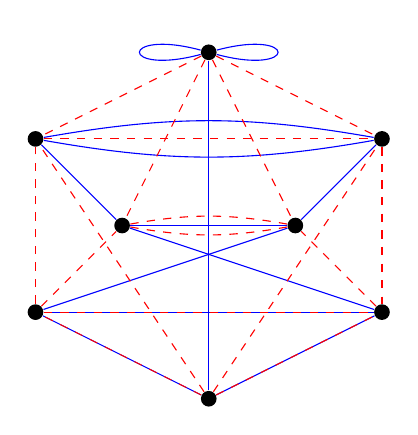
\begin{tikzpicture}[x=1.1cm,y=1.1cm]
      \begin{scope}[every node/.style={fill,black,circle,inner sep=2pt}]
        \node at (0,0)  (1){};
        \node at (0,4) (20){};
        \node at (2,1)  (16z){};
        \node at (-2,1)  (81z){};
        \node at (-1,2) (77z){};
        \node at (1,2)  (20z){};
        \node at (-2,3)  (85z){};
        \node at (2,3)  (12z){};
      \end{scope}
      
      \begin{scope}[blue,every loop/.style={looseness=50}]
        \path (1) edge (20) edge (16z) edge (81z);
        \path (20) edge[loop left] (20) edge[loop right] (20);
        \path (16z) edge (81z) edge (77z);
        \path (81z) edge (20z);
        \path (77z) edge (20z) edge (85z);
        \path (20z) edge (12z);
        \path (12z) edge[bend right=10] (85z) edge[bend left=10] (85z);
      \end{scope}
      
      \begin{scope}[red,dashed]
        \path (1) edge (85z) edge (81z) edge (12z) edge (16z);
        \path (20) edge (85z) edge (77z) edge (20z) edge (12z);
        \path (81z) edge (85z) edge (77z) edge (16z);
        \path (85z) edge (12z);
        \path (12z) edge (16z);
        \path (16z) edge (20z);
        \path (20z) edge[bend right=10] (77z) edge[bend left=10] (77z);
      \end{scope}
    \end{tikzpicture}
    \caption{The supersingular isogeny graphs of degree 2
      (blue, continuous) and 3 (red, dashed) on $\F_{97^2}$.}
    \label{fig:sidh}
  \end{minipage}
  \hfill
  \begin{minipage}{0.47\textwidth}
    \centering
    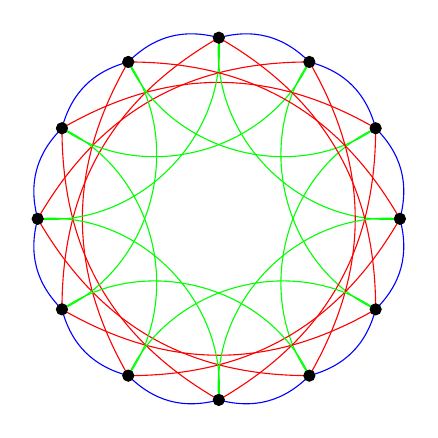
\begin{tikzpicture}
      \def\crater{12}
      \def\jumpa{-8}
      \def\jumpb{9}
      \def\diam{2.3cm}

      \foreach \i in {1,...,\crater} {
        \draw[blue] (360/\crater*\i : \diam) to[bend right] (360/\crater*\i+360/\crater : \diam);
        \draw[red] (360/\crater*\i : \diam) to[bend right] (360/\crater*\i+\jumpa*360/\crater : \diam);
        \draw[green] (360/\crater*\i : \diam) to[bend right=50] (360/\crater*\i+\jumpb*360/\crater : \diam);
      }
      \foreach \i in {1,...,\crater} {
        \pgfmathparse{int(mod(2^\i,13))}
        \let\exp\pgfmathresult
        \draw[fill] (360/\crater*\i: \diam) circle (2pt);
      }
    \end{tikzpicture}
    \caption{The supersingular isogeny graphs of degree 3 (blue), 5
      (red) and 7 (green), restricted to $\F_{89}$-rational
      isomorphism classes.\\
      Also the connected component of $j=77$ in the ordinary isogeny
      graph of $\F_{233}$ (same isogeny degrees).}
    \label{fig:csidh}
  \end{minipage}
\end{figure}



The fundamental theorem of complex multiplication gifts us with a
regular group action of a finite abelian group onto a finite set. %
Moreover, both the group and the set are easy to instantiate, and
their sizes can be controlled to a certain extent. %


\section{Cryptographic group actions}
It is natural to ask to what extent public key cryptography can be
founded upon group actions, a question first explored by Brassard and
Yung in the early 90's~\cite{C:BraYun90}. %
Drawing inspiration from the complex multiplication group action,
Couveignes formalized the concept of \emph{Hard Homogeneous Space}.%
\footnote{In topology, a \emph{homogeneous space} for a group $G$ is a
  space $X$ such that $G$ acts transitively on it.} %
Couveignes' definition was recently refined in~\cite{AC:ADMP20}, whose
terminology we are going to borrow to present the cryptographic
applications of complex multiplication isogeny graphs.

\begin{definition}[Effective Group Action]
  A group action $(G,X,\star )$ is \emph{effective} if the following
  properties are satisfied:
  \begin{enumerate}
  \item The group $G$ is finite and there exist efficient algorithms
    for:
    \begin{enumerate}
    \item \emph{Membership testing}, i.e., to decide if a given bit string
      represents a valid group element in $G$.
    \item \emph{Equality testing}, i.e., to decide if two bit strings
      represent the same group element in $G$.
    \item \emph{Sampling}, i.e., to sample an element $g$ from a
      distribution on $G$ statistically close to uniform.
    \item \emph{Operation}, i.e., to compute $gh$ for any $g,h\in G$.
    \item \emph{Inversion}, i.e., to compute $g^{-1}$ for any
      $g\in G$.
    \end{enumerate}
  \item The set $X$ is finite and there exist efficient algorithms for:
    \begin{enumerate}
    \item \emph{Membership testing}, i.e., to decide if a bit string
      represents a valid set element.
    \item \emph{Unique representation}, i.e., given any arbitrary set element $x\in X$, compute a string $\hat{x}$ that canonically represents $x$.
    \end{enumerate}
  \item There exists a distinguished element $x_0\in X$, called the
    \emph{origin}, such that its bit-string representation is known.
  \item There exists an efficient algorithm that given (some
    bit-string representations of) any $g\in G$ and any $x\in X$,
    outputs $g \star x$.
  \end{enumerate}
\end{definition}

\begin{definition}[Restricted Effective Group Action]
  Let $(G,X,\star )$ be a group action and let $\vec{g} =(g_1,\ldots,g_n)$
  be a (not necessarily minimal) generating set for $G$.  The action
  is said to be \emph{$\vec{g}$-restricted effective}, if the
  following properties are satisfied:
  \begin{enumerate}
  \item $G$ is finite and $n = \polylog(\abs{G})$.
  \item The set $X$ is finite and there exist efficient algorithms
    for: \emph{Membership testing}, i.e., to decide if a bit string
    represents a valid set element; and \emph{Unique representation},
    i.e., to compute a string $\hat{x}$ that canonically represents
    any given set element $x\in X$.
  \item There exists a distinguished element $x_0\in X$, called the
    \emph{origin}, such that its bit-string representation is known.
  \item There exists an efficient algorithm that given any
    $1\le i\le n$ and any bit string representation of $x\in X$,
    outputs $g_i\star x$ and $g_i^{-1}\star x$.
  \end{enumerate}
\end{definition}

The two definitions above, which will be referred to by the intialisms
EGA and REGA, describe the algorithmic properties we expect from a
cryptographically useful group action. %
EGAs are simpler to work with, and closely match the original
definitions of Brassard, Yung and Couveignes, but they imperfectly
model the properties of the complex multiplication group action, for
which REGA is a better model. %
Besides the algorithmic properties, we shall need some computational
assumptions to work with group actions.

\begin{definition}
  Let $(G,X, \star )$ be a group action. %
  Suppose that the functions $f_x$ and the permutations $\pi_g$
  defined by
  \begin{equation*}
    \begin{aligned}
      f_x : G &\to X,\\
      g &\mapsto g\star x,
    \end{aligned}
    \qquad\qquad
    \begin{aligned}
      \pi_g : X &\to X,\\
      x &\mapsto g\star x.
    \end{aligned}
  \end{equation*}
  are efficiently computable for any $x\in X$ and $g\in G$. %
  The group action is said to be:
  \begin{enumerate}
  \item \emph{One-way} if the family of functions $f_x$ is one-way.
  \item \emph{Weakly unpredictable} if the family of permutations
    $\pi_g$ is weakly unpredictable, i.e., if given a list of random
    pairs $(x,\pi_g(x))$ it is hard to guess $\pi_g(x^*)$ for a random
    $x^*$ not in the list.
  \item \emph{Weakly pseudorandom} if the family of permutations
    $\pi_g$ is weakly pseudorandom, i.e., if it is hard to distinguish
    between a list of random pairs $(x,\pi_g(x))$ and one of random
    pairs $(x,\pi(x))$, where $\pi$ is a uniformly drawn permutation
    of $X$.
  \end{enumerate}
\end{definition}

These definitions generalize classical discrete logarithm based
cryptography. %
Indeed, if $G$ is an effective cyclic group of order $p$, it is easily
verified that the action of $(\Z/p\Z)^\times$ on $G$ defined by
$a\star g = g^a$ is an EGA, and that one wayness, weak
unpredictability and weak pseudorandomness correspond to the hardness
of, respectively, DLP, CDH and DDH.

- key exchange

- ZK, signatures

- other stuff

- non generic stuff

\section{The full supersingular graph and SIDH}

- GPST attack
- ZK

\section{The endomorphism ring as a trapdoor}

- KLPT, torsion point attacks, reduction to End
- S�ta, GPS, SQISign

\section{Isogeny computations and time delay protocols}

- V�lu, etc.
- VDF, DE

\section{Some open problems}

- Pedersen: Hashing, HE
- Impl, side channel


%%% Local Variables:
%%% mode: latex
%%% TeX-master: "main"
%%% End:

% LocalWords:  isogeny additively morphisms morphism supersingular
% LocalWords:  isogenies undirected expander quaternion endomorphism
% LocalWords:  monic Cayley discriminants inhomogeneous instantiation
% LocalWords:  homomorphic cryptographic cryptosystems reducibility
% LocalWords:  cryptographically EGA REGA EGAs
